\documentclass{_mypackages/monograph}

\title{Formation and Evolution of Galaxies \\ Problem Set 04 \\ Formation of Structures} % \MyTitle
\author{Bruno Murino - 8944901} % \MyAuthor
\date{\today} % \MyDate

\addbibresource{qinfo.bib}
\graphicspath{ {figures/} }

\begin{document}
% \frontmatter

\solutionstp
% \dominitoc
% \doparttoc
% \pagestyle{onlypagenum}
% \tableofcontents
% \mainmatter

\subsubsection{1)}

\begin{figure}[H]
    \centering
    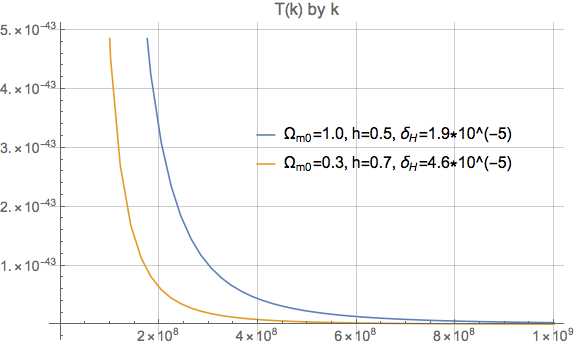
\includegraphics[width=0.8\textwidth]{tkbyk.png}
    \caption{Plot of the Power Spectrum.}
    \label{fig:tkbyk}
\end{figure}

\begin{figure}[H]
    \centering
    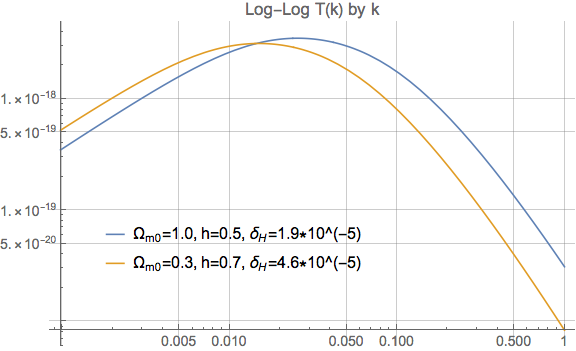
\includegraphics[width=0.8\textwidth]{loglogtkbyk.png}
    \caption{Log-Log Plot of the Power Spectrum.}
    \label{fig:loglogtkbyk}
\end{figure}

\paragraph{c)}

Looking at the figures above we can see that for \(k\gg 1\) we find the expected behaviour \(T(k) \sim k^{-2}\). However, for \(k \ll 1\) we expected to see, on the log-log plot, a constant curve near \(0\) but this was not observed.





\subsubsection{2)}

The comoving radius \(\omega(t)\) is given by
\begin{equation}
    \omega(t) = \int_0^{t} \dd{r} = \int_0^{t} \frac{c}{a(t')} \dd{t'},
\end{equation}
which we can change variables from \(t'\) to \(a(t')\) using the fact that
\begin{equation}
    \dv{t} a(t) = \dot{a}(t) \qq{implies} \dd{t} = \frac{1}{\dot{a}}\dd{a},
\end{equation}
to find
\begin{equation}\label{eq:generalcomrad}
    \omega(t) = c \int_0^{a(t)} \frac{\dd{a}}{a\dot{a}}.
\end{equation}

From the Big Bang to the recombination epoch we can consider a matter dominated evolution, meaning that
\begin{equation}
    a\dot{a} = H_0 \sqrt{\Omega_{m,0}} \sqrt{a},
\end{equation}
which we can plug into \eqref{eq:generalcomrad} to find
\begin{equation}
    \omega(t) = \frac{c}{H_0\sqrt{\Omega_{m,0}}} \int_0^{a(t)} \frac{\dd{a}}{\sqrt{a}},
\end{equation}
and since
\begin{equation}
    \int_0^{a(t)} \frac{\dd{a}}{\sqrt{a}} = \eval{2\sqrt{a(t')}}_0^{a(t)} = 2\sqrt{a(t)},
\end{equation}
we find that
\begin{equation}\label{eq:comradatrecom}
    \omega(t) = \frac{2c\sqrt{a(t)}}{H_0\sqrt{\Omega_{m,0}}}\qc t \in T_\text{Recombination epoch}.
\end{equation}
If \(t \in T_\text{Recombination epoch}\), then let's denote \(t=t_\text{rec}\).

We know that the redshift for the recombination epoch is around \(z\sim 1100\), which implies that the scale factor at the recombination epoch was
\begin{equation}\label{eq:scalefacatrec}
    a(t_\text{rec}) = \frac{1}{1+z} = \frac{1}{1+1100} \approx \frac{1}{1100}.
\end{equation}

Plugging \eqref{eq:scalefacatrec} on \eqref{eq:comradatrecom}, and considering \(\Omega_{m,0}=1\), we find
\begin{equation}
    \omega(t_\text{rec}) \approx 180\, h^{-1}\, \si{\mega\parsec} \approx  \SI{257}{\mega\parsec},
\end{equation}
considering \(h=0.7\).

\subsubsection{3)}

The Press-Schechter mass function is
\begin{equation}\label{eq:PSmassfunc}
    n(M) = \frac{2}{\sqrt{\pi}} \frac{\alpha \overline{\rho}}{M^2} \left( \frac{M}{M_*} \right)^\alpha \lexp\Big[ - \left( \frac{M}{M_*}\right)^{2\alpha} \Big]\qc \alpha = \frac{3+n}{6}.
\end{equation}
If
\begin{equation}
    \frac{L}{L_*} = \bigg(\frac{M}{M_*}\bigg)^{2\alpha},
\end{equation}
then we can rewrite \eqref{eq:PSmassfunc} as 
\begin{equation}
    n'(L) = \frac{2}{\sqrt{\pi}} \frac{\alpha \overline{\rho}}{M_*^2} \left( \frac{L}{L_*} \right)^{\frac{1}{2}-\frac{1}{\alpha}} \lexp\Big[ - \frac{L}{L_*} \Big].
\end{equation}

Observations of the luminosity function yields an exponent of \(-1.25\) on the \(\nicefrac{L}{L_*}^{\nicefrac{1}{2}-\nicefrac{1}{\alpha}}\) term, meaning that we need
\begin{equation}
    -1.25 = \frac{1}{2}-\frac{1}{\alpha},
\end{equation}
implying that
\begin{equation}
    \alpha = \frac{2}{1-2*(-1.25)} = \frac{2}{3.5} = \hlf + \frac{n}{6},
\end{equation}
further implying that
\begin{equation}
    n = \frac{3}{7} \approx 0.428571.
\end{equation}






% \backmatter
% \printbib
\end{document}